%
% Einführung in die Mustererkennung - WS2013
% Abgabeprotokoll Exercise 1
%
%

%{{{ misc
\documentclass[a4paper,psfig,subfigure,epsfig,fleqn,amssmb,float,caption,fontenc,ausarbeitung]{article}

\usepackage{graphicx}
\usepackage{caption}
\usepackage{subcaption}

\usepackage{pgfplots}

%Zitieren:
\usepackage[english]{babel}
%\usepackage[german]{babel}
\usepackage{babelbib} % für das Erstellen des Bibtex-Literaturverzeichnisses
\usepackage{cite}
%\selectbiblanguage{english}
%\selectbiblanguage{german}


\usepackage{url}

\usepackage[]{mcode}

\usepackage[pdftitle={Einfuehrung in die Mustererkennung, Exercise 1},
            pdfauthor={David Pfahler},
						pdfauthor={Matthias Gusenbauer},
						pdfauthor={Matthias Vigele},
            pdfsubject={Mustererkennung},
            pdfborder={0 0 0}]{hyperref}


%%%%%%%%%%%%%%%%%%%%%%%%%%%%%%%%
% Titlepage

\pagestyle{empty}


%set dimensions of columns, gap between columns, and paragraph indent

\setlength{\textheight}{24.7 cm}
\setlength{\columnsep}{1 cm}
\setlength{\textwidth}{16 cm}
%\setlength{\footheight}{0.0 cm}
\setlength{\topmargin}{0.0 cm}
\setlength{\headheight}{0.0 cm}
\setlength{\headsep}{-0.3 cm}
\setlength{\oddsidemargin}{0.0 cm}
\setlength{\parindent}{0.7 cm}
\setlength{\mathindent}{0mm}

% set page counter if document is part of proceedings
\setcounter{page}{1}
\renewcommand{\floatpagefraction}{0.9}
\renewcommand{\textfraction}{0.1}

%\renewcommand{\captionlabelfont}{\fontfamily{phv}\fontseries{bx}\fontsize{10}{10pt}\selectfont}
%\renewcommand{\captionfont}{\fontfamily{phv}\fontsize{10}{12pt}\selectfont}
%\setlength{\captionmargin}{0.5 cm}

\makeatletter
\makeatother
\def\RR{\hbox{I\kern-.2em\hbox{R}}}


\begin{document}

%don't want date printed
\date{}

%make title bold and 14 pt font (Latex default is non-bold, 16pt) 
\title{~\\
  ~\\
  \fontsize{14}{14pt} \bf Abgabedokument Exercise 1
	 ~\\
  \fontsize{12}{12pt} \bf Einführung in die Mustererkennung 186.840 WS 2013}

%for single author 
\author{~\\
  ~\\
  \fontsize{12}{12pt}
  {\bf David Pfahler, Matthias Gusenbauer, Matthias Vigele}\\
  1126287, 1125577, 1126171
  ~\\ ~\\ ~\\
  \normalsize
  {\bf ABSTRACT} \\ 
  \noindent
  \hspace{0.2cm}
  \begin{minipage}[c]{15cm}
  \normalsize This is my abstract.  This is my abstract.  This is my
    abstract.  This is my abstract.  This is my abstract.  This is my
    abstract.  This is my abstract.  This is my abstract.  This is my
    abstract.  This is my abstract.  This is my abstract.  This is my
    abstract.\\
  \end{minipage}
  ~\\ ~\\ ~\\
  \normalsize
  {\bf KEYWORDS} \\ 
  \normalsize
  Keyword1, Keyword2, Keyword3, Keyword4, Keyword5, Keyword6.
  }

\maketitle
%I don't know why I have to reset thispagestyle, but otherwise get page numbers 
\normalfont
\thispagestyle{empty}

%%%%%%%%%%%%%%%%%%%%%%%%%%%%%%%%%%%%%%%%%%%%%%%%%%%%%%%%%%%%%%%%%%%%%%%%%%%%%%%%
% CONTENT

\section{Feature Extraction}
\label{sec:featureExtraction}

This section describes the used image classes and the features that are used for the classification (see Section \ref{sec:classification}. 

\subsection{Input Images}
\label{sec:input}

5 Classes from the MPEG7 CE-Shape-1 database \cite{latecki2000shape} are used. We used:

\begin{itemize}
	\item Heart
	\item device4
	\item bat
	\item device1
	\item Bone
\end{itemize}

Figure \ref{fig:classes} shows example images of the used classes.

\begin{figure}
	\centering
	\begin{subfigure}[b]{0.3\textwidth}
		\includegraphics[width=\textwidth]{img/Heart-1}
		\caption{Heart}
	\end{subfigure}
	~ 
	\begin{subfigure}[b]{0.3\textwidth}
		
\includegraphics[width=\textwidth]{img/Bone}
		\caption{Bone}
	\end{subfigure}
	~
	\begin{subfigure}[b]{0.3\textwidth}
		
\includegraphics[width=\textwidth]{img/device1}
		\caption{device1}
	\end{subfigure}
	~
	\begin{subfigure}[b]{0.3\textwidth}
		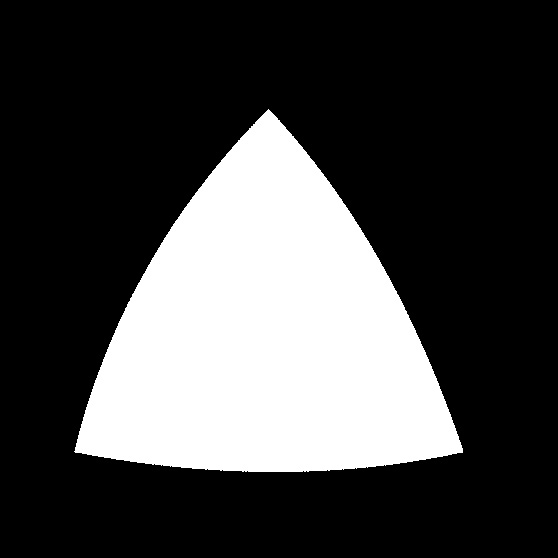
\includegraphics[width=\textwidth]{img/device4}
		\caption{device4}
	\end{subfigure}
	~
	\begin{subfigure}[b]{0.3\textwidth}
		
\includegraphics[width=\textwidth]{img/bat}
		\caption{bat}
	\end{subfigure}
	~
	\caption{5 used Classes from the MPEG7 CE-Shape-1 database \cite{latecki2000shape}}
	\label{fig:classes}
\end{figure}


\subsection{Features}
\label{sec:features}

In the following section the used features are described. To evaluate scale, 
transformation and rotation invariants a test image is used. Listing 
\ref{lst:calcRot} shows the used matlab function. Figure \ref{fig:heart} 
shows the test image. 

\begin{lstlisting}[caption=Calculate rotated image, label=lst:calcRot]
	rot = imresize(imrotate(image,45),0.5);
\end{lstlisting}
The calculation of the features of the two test images will differ, because 
of the lost of accuracy by the size reduction.

\subsubsection{Eccentricity}
\label{sec:eccentricity}

The Eccentricity is a scalar value that measures of how much the object 
deviates from a circle. It is calculated by the ratio of the distance between 
the foci of the ellipse and its major axis length. See Equation 
\ref{eq:eccentricity}
\begin{equation}
	\frac{2*\sqrt{\frac{D_{max}}{2}^2-\frac{D_{min}}{2}^2}}{D_{max}}
	\label{eq:eccentricity}
\end{equation}
$D_{max}$ is the major axis length and $D_{min}$ is the minor axis length of 
the best-fit ellipse.

\paragraph{Invariance:} The eccentricity feature is scale, transformation and 
rotation invariant. The Listing \ref{lst:eccentricity} provides an example. 
Figure \ref{fig:heart} shows the used binary images.

\begin{lstlisting}[caption=Calculate eccentricity in matlab, label=lst:eccentricity]
>> regionprops(image,'Eccentricity')

ans = 

    Eccentricity: 0.7073

>> regionprops(rot,'Eccentricity')

ans = 

    Eccentricity: 0.7080
\end{lstlisting}

\subsubsection{Roundness}
\label{sec:roundness}

Roundness is a scalar value that describe how the shape of an object 
approaches that of a circle. A value of 1 means that the object is a circle 
and a value of 0 means the object is a line segment. See Equation \ref{eq:roundness}
\begin{equation}
  \frac{4A(R)}{\pi D^{2}_{max}}
	\label{eq:roundness}
\end{equation}
$A(R)$ is the area of the labeled binary image and $D_{max}$ is the major axis 
length of the best-fit ellipse.

\paragraph{Invariance:} The Roundness feature is scale, transformation and 
rotation invariant. The Listing \ref{lst:roundness} provides an example. 
Figure \ref{fig:heart} shows the used binary images.

\begin{lstlisting}[caption=Calculate roundness in matlab, label=lst:roundness]
	>> calculateRoundness(image)

	ans = 

			Roundness: 0.6333
	
	>> calculateRoundness(rot)

	ans = 

			Roundness: 0.6326
\end{lstlisting}

\begin{figure}
	\centering
	\begin{subfigure}[b]{0.4\textwidth}
		
\includegraphics[width=\textwidth]{img/heart.jpg}
	\end{subfigure}
	~ 
	\begin{subfigure}[b]{0.4\textwidth}
		
\includegraphics[width=\textwidth]{img/invariance_rotation.jpg}
	\end{subfigure}
	\caption{A rotated, translated and scaled image}
	\label{fig:heart}
\end{figure}


\subsubsection{Solidity}
\label{sec:solidity}

The solidity is a scalar value specifying the proportion of the pixels in the 
convex hull that are also in the region. See Equation \ref{eq:solidity}

\begin{equation}
\frac{A(R)}{A(Co(R))}
\label{eq:solidity}
\end{equation}
$A(R)$ is the area of the labeled binary image and $Co(R)$ is the convex hull of the binary image

\paragraph{Invariance:} The solidity feature is scale, transformation and 
rotation invariant. The Listing \ref{lst:solidity} provides an example. 
Figure \ref{fig:heart} shows the used binary images.
\begin{lstlisting}[caption=Calculate solidity in matlab, label=lst:solidity]
>> regionprops(image,'Solidity')

ans = 

    Solidity: 0.9145

>> regionprops(rot,'Solidity')

ans = 

    Solidity: 0.9113
\end{lstlisting}

\subsection{Results}
\label{sec:fResults}

With the {\tt matlab} function {\tt getFeatures} all features for all input 
images (see Section \ref{sec:input}) are calculated. In Figure \ref{fig:boxplot} 
a boxplot  of this features is shown. The boxplot is a convenient way of 
graphically depicting groups of numerical data through their quartiles. 
\cite{tukey1977exploratory}
The Figure \ref{fig:gscatter} shows the dependencies of all features and displays outliers.

\begin{figure}
	\centering
	\newlength\figureheight 
	\newlength\figurewidth 
	\setlength\figureheight{6cm} 
	\setlength\figurewidth{10cm}
	% This file was created by matlab2tikz v0.4.3.
% Copyright (c) 2008--2013, Nico Schlömer <nico.schloemer@gmail.com>
% All rights reserved.
% 
% The latest updates can be retrieved from
%   http://www.mathworks.com/matlabcentral/fileexchange/22022-matlab2tikz
% where you can also make suggestions and rate matlab2tikz.
% 
\begin{tikzpicture}

\begin{axis}[%
width=4.553125in,
height=2.19734064736561in,
unbounded coords=jump,
scale only axis,
xmin=0.5,
xmax=5.5,
xtick={\empty},
ymin=0.0332958833271357,
ymax=1.00818584326667,
name=plot2,
title={Roundness}
]
\addplot [
color=black,
dashed,
forget plot
]
table[row sep=crcr]{
1 0.651495725539113\\
1 0.710554628449968\\
};
\addplot [
color=black,
dashed,
forget plot
]
table[row sep=crcr]{
2 0.795527595089137\\
2 0.890375569661562\\
};
\addplot [
color=black,
dashed,
forget plot
]
table[row sep=crcr]{
3 0.30337788305282\\
3 0.336818908570996\\
};
\addplot [
color=black,
dashed,
forget plot
]
table[row sep=crcr]{
4 0.916849176057055\\
4 0.963872663269414\\
};
\addplot [
color=black,
dashed,
forget plot
]
table[row sep=crcr]{
5 0.0941369583883711\\
5 0.0969134217023442\\
};
\addplot [
color=black,
dashed,
forget plot
]
table[row sep=crcr]{
1 0.524181574417953\\
1 0.577932520150441\\
};
\addplot [
color=black,
dashed,
forget plot
]
table[row sep=crcr]{
2 0.575268759243766\\
2 0.653414764221894\\
};
\addplot [
color=black,
dashed,
forget plot
]
table[row sep=crcr]{
3 0.16439260714369\\
3 0.224508500687679\\
};
\addplot [
color=black,
dashed,
forget plot
]
table[row sep=crcr]{
4 0.82676790703128\\
4 0.826960701954154\\
};
\addplot [
color=black,
dashed,
forget plot
]
table[row sep=crcr]{
5 0.0776090633243871\\
5 0.0844090063349556\\
};
\addplot [
color=black,
solid,
forget plot
]
table[row sep=crcr]{
0.875 0.710554628449968\\
1.125 0.710554628449968\\
};
\addplot [
color=black,
solid,
forget plot
]
table[row sep=crcr]{
1.875 0.890375569661562\\
2.125 0.890375569661562\\
};
\addplot [
color=black,
solid,
forget plot
]
table[row sep=crcr]{
2.875 0.336818908570996\\
3.125 0.336818908570996\\
};
\addplot [
color=black,
solid,
forget plot
]
table[row sep=crcr]{
3.875 0.963872663269414\\
4.125 0.963872663269414\\
};
\addplot [
color=black,
solid,
forget plot
]
table[row sep=crcr]{
4.875 0.0969134217023442\\
5.125 0.0969134217023442\\
};
\addplot [
color=black,
solid,
forget plot
]
table[row sep=crcr]{
0.875 0.524181574417953\\
1.125 0.524181574417953\\
};
\addplot [
color=black,
solid,
forget plot
]
table[row sep=crcr]{
1.875 0.575268759243766\\
2.125 0.575268759243766\\
};
\addplot [
color=black,
solid,
forget plot
]
table[row sep=crcr]{
2.875 0.16439260714369\\
3.125 0.16439260714369\\
};
\addplot [
color=black,
solid,
forget plot
]
table[row sep=crcr]{
3.875 0.82676790703128\\
4.125 0.82676790703128\\
};
\addplot [
color=black,
solid,
forget plot
]
table[row sep=crcr]{
4.875 0.0776090633243871\\
5.125 0.0776090633243871\\
};
\addplot [
color=blue,
solid,
forget plot
]
table[row sep=crcr]{
0.75 0.577932520150441\\
0.75 0.651495725539113\\
1.25 0.651495725539113\\
1.25 0.577932520150441\\
0.75 0.577932520150441\\
};
\addplot [
color=blue,
solid,
forget plot
]
table[row sep=crcr]{
1.75 0.653414764221894\\
1.75 0.795527595089137\\
2.25 0.795527595089137\\
2.25 0.653414764221894\\
1.75 0.653414764221894\\
};
\addplot [
color=blue,
solid,
forget plot
]
table[row sep=crcr]{
2.75 0.224508500687679\\
2.75 0.30337788305282\\
3.25 0.30337788305282\\
3.25 0.224508500687679\\
2.75 0.224508500687679\\
};
\addplot [
color=blue,
solid,
forget plot
]
table[row sep=crcr]{
3.75 0.826960701954154\\
3.75 0.916849176057055\\
4.25 0.916849176057055\\
4.25 0.826960701954154\\
3.75 0.826960701954154\\
};
\addplot [
color=blue,
solid,
forget plot
]
table[row sep=crcr]{
4.75 0.0844090063349556\\
4.75 0.0941369583883711\\
5.25 0.0941369583883711\\
5.25 0.0844090063349556\\
4.75 0.0844090063349556\\
};
\addplot [
color=red,
solid,
forget plot
]
table[row sep=crcr]{
0.75 0.618827184406748\\
1.25 0.618827184406748\\
};
\addplot [
color=red,
solid,
forget plot
]
table[row sep=crcr]{
1.75 0.715017194567567\\
2.25 0.715017194567567\\
};
\addplot [
color=red,
solid,
forget plot
]
table[row sep=crcr]{
2.75 0.286542191156502\\
3.25 0.286542191156502\\
};
\addplot [
color=red,
solid,
forget plot
]
table[row sep=crcr]{
3.75 0.861182521224414\\
4.25 0.861182521224414\\
};
\addplot [
color=red,
solid,
forget plot
]
table[row sep=crcr]{
4.75 0.0868883401760468\\
5.25 0.0868883401760468\\
};
\addplot [
color=blue,
only marks,
mark=+,
mark options={solid,draw=red},
forget plot
]
table[row sep=crcr]{
1 0.791065911400579\\
};


\addplot [
color=blue,
only marks,
mark=+,
mark options={solid,draw=red},
forget plot
]
table[row sep=crcr]{
4 0.576417890052189\\
4 0.578053097415167\\
4 0.579091704656874\\
4 0.685232434045994\\
};
\addplot [
color=blue,
only marks,
mark=+,
mark options={solid,draw=red},
forget plot
]
table[row sep=crcr]{
5 0.124579759131964\\
5 0.128887707033575\\
5 0.154563596450397\\
};
\end{axis}

\begin{axis}[%
width=4.553125in,
height=2.08139228886169in,
unbounded coords=jump,
scale only axis,
xmin=0.5,
xmax=5.5,
xtick={\empty},
ymin=0.0243256276331408,
ymax=1.04049898029786,
at=(plot2.above north west),
anchor=below south west,
title={Eccentricity}
]
\addplot [
color=black,
dashed,
forget plot
]
table[row sep=crcr]{
1 0.737188234680554\\
1 0.816086325006819\\
};
\addplot [
color=black,
dashed,
forget plot
]
table[row sep=crcr]{
2 0.379862033488001\\
2 0.44867774521782\\
};
\addplot [
color=black,
dashed,
forget plot
]
table[row sep=crcr]{
3 0.911170985338075\\
3 0.924570454993097\\
};
\addplot [
color=black,
dashed,
forget plot
]
table[row sep=crcr]{
4 0.135891252162863\\
4 0.193575729182042\\
};
\addplot [
color=black,
dashed,
forget plot
]
table[row sep=crcr]{
5 0.987540085244819\\
5 0.994309282449462\\
};
\addplot [
color=black,
dashed,
forget plot
]
table[row sep=crcr]{
1 0.640019004957429\\
1 0.680441483157064\\
};
\addplot [
color=black,
dashed,
forget plot
]
table[row sep=crcr]{
2 0.165371273657048\\
2 0.214184643976312\\
};
\addplot [
color=black,
dashed,
forget plot
]
table[row sep=crcr]{
3 0.874845865471273\\
3 0.890253697229678\\
};
\addplot [
color=black,
dashed,
forget plot
]
table[row sep=crcr]{
4 0.0705153254815371\\
4 0.0944930658447764\\
};
\addplot [
color=black,
dashed,
forget plot
]
table[row sep=crcr]{
5 0.974829939696739\\
5 0.980546207571909\\
};
\addplot [
color=black,
solid,
forget plot
]
table[row sep=crcr]{
0.875 0.816086325006819\\
1.125 0.816086325006819\\
};
\addplot [
color=black,
solid,
forget plot
]
table[row sep=crcr]{
1.875 0.44867774521782\\
2.125 0.44867774521782\\
};
\addplot [
color=black,
solid,
forget plot
]
table[row sep=crcr]{
2.875 0.924570454993097\\
3.125 0.924570454993097\\
};
\addplot [
color=black,
solid,
forget plot
]
table[row sep=crcr]{
3.875 0.193575729182042\\
4.125 0.193575729182042\\
};
\addplot [
color=black,
solid,
forget plot
]
table[row sep=crcr]{
4.875 0.994309282449462\\
5.125 0.994309282449462\\
};
\addplot [
color=black,
solid,
forget plot
]
table[row sep=crcr]{
0.875 0.640019004957429\\
1.125 0.640019004957429\\
};
\addplot [
color=black,
solid,
forget plot
]
table[row sep=crcr]{
1.875 0.165371273657048\\
2.125 0.165371273657048\\
};
\addplot [
color=black,
solid,
forget plot
]
table[row sep=crcr]{
2.875 0.874845865471273\\
3.125 0.874845865471273\\
};
\addplot [
color=black,
solid,
forget plot
]
table[row sep=crcr]{
3.875 0.0705153254815371\\
4.125 0.0705153254815371\\
};
\addplot [
color=black,
solid,
forget plot
]
table[row sep=crcr]{
4.875 0.974829939696739\\
5.125 0.974829939696739\\
};
\addplot [
color=blue,
solid,
forget plot
]
table[row sep=crcr]{
0.75 0.680441483157064\\
0.75 0.737188234680554\\
1.25 0.737188234680554\\
1.25 0.680441483157064\\
0.75 0.680441483157064\\
};
\addplot [
color=blue,
solid,
forget plot
]
table[row sep=crcr]{
1.75 0.214184643976312\\
1.75 0.379862033488001\\
2.25 0.379862033488001\\
2.25 0.214184643976312\\
1.75 0.214184643976312\\
};
\addplot [
color=blue,
solid,
forget plot
]
table[row sep=crcr]{
2.75 0.890253697229678\\
2.75 0.911170985338075\\
3.25 0.911170985338075\\
3.25 0.890253697229678\\
2.75 0.890253697229678\\
};
\addplot [
color=blue,
solid,
forget plot
]
table[row sep=crcr]{
3.75 0.0944930658447764\\
3.75 0.135891252162863\\
4.25 0.135891252162863\\
4.25 0.0944930658447764\\
3.75 0.0944930658447764\\
};
\addplot [
color=blue,
solid,
forget plot
]
table[row sep=crcr]{
4.75 0.980546207571909\\
4.75 0.987540085244819\\
5.25 0.987540085244819\\
5.25 0.980546207571909\\
4.75 0.980546207571909\\
};
\addplot [
color=red,
solid,
forget plot
]
table[row sep=crcr]{
0.75 0.708305903154552\\
1.25 0.708305903154552\\
};
\addplot [
color=red,
solid,
forget plot
]
table[row sep=crcr]{
1.75 0.310368368614242\\
2.25 0.310368368614242\\
};
\addplot [
color=red,
solid,
forget plot
]
table[row sep=crcr]{
2.75 0.901148318863892\\
3.25 0.901148318863892\\
};
\addplot [
color=red,
solid,
forget plot
]
table[row sep=crcr]{
3.75 0.115700129581742\\
4.25 0.115700129581742\\
};
\addplot [
color=red,
solid,
forget plot
]
table[row sep=crcr]{
4.75 0.985466357631359\\
5.25 0.985466357631359\\
};
\addplot [
color=blue,
only marks,
mark=+,
mark options={solid,draw=red},
forget plot
]
table[row sep=crcr]{
1 0.470102007919441\\
};
\addplot [
color=blue,
only marks,
mark=+,
mark options={solid,draw=red},
forget plot
]
table[row sep=crcr]{
3 0.81603423066178\\
3 0.816048286890373\\
3 0.944446119170283\\
3 0.944452016765911\\
};
\end{axis}

\begin{axis}[%
width=4.553125in,
height=2.26614191026485in,
unbounded coords=jump,
scale only axis,
xmin=0.5,
xmax=5.5,
xtick={\empty},
ymin=0.35240496529994,
ymax=1.02568973900425,
at=(plot2.below south west),
anchor=above north west,
title={Solidity}
]
\addplot [
color=black,
dashed,
forget plot
]
table[row sep=crcr]{
1 0.914303058840295\\
1 0.948246659557117\\
};
\addplot [
color=black,
dashed,
forget plot
]
table[row sep=crcr]{
2 0.910704046222787\\
2 0.995085885654052\\
};
\addplot [
color=black,
dashed,
forget plot
]
table[row sep=crcr]{
3 0.687199446149801\\
3 0.710613192129176\\
};
\addplot [
color=black,
dashed,
forget plot
]
table[row sep=crcr]{
4 0.753375165861245\\
4 0.863805831954767\\
};
\addplot [
color=black,
dashed,
forget plot
]
table[row sep=crcr]{
5 0.537128019294235\\
5 0.618302057427086\\
};
\addplot [
color=black,
dashed,
forget plot
]
table[row sep=crcr]{
1 0.815341397695351\\
1 0.868411919619642\\
};
\addplot [
color=black,
dashed,
forget plot
]
table[row sep=crcr]{
2 0.751066645230705\\
2 0.785774109719246\\
};
\addplot [
color=black,
dashed,
forget plot
]
table[row sep=crcr]{
3 0.46697653561912\\
3 0.577590356695149\\
};
\addplot [
color=black,
dashed,
forget plot
]
table[row sep=crcr]{
4 0.526102151516255\\
4 0.628438272579906\\
};
\addplot [
color=black,
dashed,
forget plot
]
table[row sep=crcr]{
5 0.383008818650135\\
5 0.451718726018018\\
};
\addplot [
color=black,
solid,
forget plot
]
table[row sep=crcr]{
0.875 0.948246659557117\\
1.125 0.948246659557117\\
};
\addplot [
color=black,
solid,
forget plot
]
table[row sep=crcr]{
1.875 0.995085885654052\\
2.125 0.995085885654052\\
};
\addplot [
color=black,
solid,
forget plot
]
table[row sep=crcr]{
2.875 0.710613192129176\\
3.125 0.710613192129176\\
};
\addplot [
color=black,
solid,
forget plot
]
table[row sep=crcr]{
3.875 0.863805831954767\\
4.125 0.863805831954767\\
};
\addplot [
color=black,
solid,
forget plot
]
table[row sep=crcr]{
4.875 0.618302057427086\\
5.125 0.618302057427086\\
};
\addplot [
color=black,
solid,
forget plot
]
table[row sep=crcr]{
0.875 0.815341397695351\\
1.125 0.815341397695351\\
};
\addplot [
color=black,
solid,
forget plot
]
table[row sep=crcr]{
1.875 0.751066645230705\\
2.125 0.751066645230705\\
};
\addplot [
color=black,
solid,
forget plot
]
table[row sep=crcr]{
2.875 0.46697653561912\\
3.125 0.46697653561912\\
};
\addplot [
color=black,
solid,
forget plot
]
table[row sep=crcr]{
3.875 0.526102151516255\\
4.125 0.526102151516255\\
};
\addplot [
color=black,
solid,
forget plot
]
table[row sep=crcr]{
4.875 0.383008818650135\\
5.125 0.383008818650135\\
};
\addplot [
color=blue,
solid,
forget plot
]
table[row sep=crcr]{
0.75 0.868411919619642\\
0.75 0.914303058840295\\
1.25 0.914303058840295\\
1.25 0.868411919619642\\
0.75 0.868411919619642\\
};
\addplot [
color=blue,
solid,
forget plot
]
table[row sep=crcr]{
1.75 0.785774109719246\\
1.75 0.910704046222787\\
2.25 0.910704046222787\\
2.25 0.785774109719246\\
1.75 0.785774109719246\\
};
\addplot [
color=blue,
solid,
forget plot
]
table[row sep=crcr]{
2.75 0.577590356695149\\
2.75 0.687199446149801\\
3.25 0.687199446149801\\
3.25 0.577590356695149\\
2.75 0.577590356695149\\
};
\addplot [
color=blue,
solid,
forget plot
]
table[row sep=crcr]{
3.75 0.628438272579906\\
3.75 0.753375165861245\\
4.25 0.753375165861245\\
4.25 0.628438272579906\\
3.75 0.628438272579906\\
};
\addplot [
color=blue,
solid,
forget plot
]
table[row sep=crcr]{
4.75 0.451718726018018\\
4.75 0.537128019294235\\
5.25 0.537128019294235\\
5.25 0.451718726018018\\
4.75 0.451718726018018\\
};
\addplot [
color=red,
solid,
forget plot
]
table[row sep=crcr]{
0.75 0.903884645671186\\
1.25 0.903884645671186\\
};
\addplot [
color=red,
solid,
forget plot
]
table[row sep=crcr]{
1.75 0.835994165309949\\
2.25 0.835994165309949\\
};
\addplot [
color=red,
solid,
forget plot
]
table[row sep=crcr]{
2.75 0.643980101182019\\
3.25 0.643980101182019\\
};
\addplot [
color=red,
solid,
forget plot
]
table[row sep=crcr]{
3.75 0.683653954366672\\
4.25 0.683653954366672\\
};
\addplot [
color=red,
solid,
forget plot
]
table[row sep=crcr]{
4.75 0.47390281585148\\
5.25 0.47390281585148\\
};
\addplot [
color=blue,
only marks,
mark=+,
mark options={solid,draw=red},
forget plot
]
table[row sep=crcr]{
2 0.470003065176805\\
2 0.471075877058545\\
2 0.478714334432193\\
};
\addplot [
color=blue,
only marks,
mark=+,
mark options={solid,draw=red},
forget plot
]
table[row sep=crcr]{
4 0.431959663620809\\
4 0.434520125717475\\
4 0.434771254532094\\
};
\addplot [
color=blue,
only marks,
mark=+,
mark options={solid,draw=red},
forget plot
]
table[row sep=crcr]{
5 0.708667905323532\\
};
\end{axis}
\end{tikzpicture}%
	\caption{Boxplot of all features}
	\label{fig:boxplot}
\end{figure}

\begin{figure}
	\centering
	\setlength\figureheight{4cm} 
	\setlength\figurewidth{10cm}
	% This file was created by matlab2tikz v0.4.3.
% Copyright (c) 2008--2013, Nico Schlömer <nico.schloemer@gmail.com>
% All rights reserved.
% 
% The latest updates can be retrieved from
%   http://www.mathworks.com/matlabcentral/fileexchange/22022-matlab2tikz
% where you can also make suggestions and rate matlab2tikz.
% 
%
% defining custom colors
\definecolor{mycolor1}{rgb}{0.8,1,0}%
\definecolor{mycolor2}{rgb}{0,1,0.4}%
\definecolor{mycolor3}{rgb}{0,0.4,1}%
\definecolor{mycolor4}{rgb}{0.800000000000001,0,1}%
%
\begin{tikzpicture}

\begin{axis}[%
width=\figurewidth,
height=\figureheight,
scale only axis,
xmin=0,
xmax=1.04430928244946,
xlabel={Eccentricity},
ymin=0,
ymax=1,
ylabel={Solidity},
name=plot2,
axis x line*=bottom,
axis y line*=left,
legend style={at={(1.03,0.5)},anchor=west,draw=black,fill=white,legend cell align=left}
]
\addplot [
color=red,
mark size=2.5pt,
only marks,
mark=*,
mark options={solid}
]
table[row sep=crcr]{
0.707288857832556 0.914473684210526\\
0.670399243226584 0.898516608104132\\
0.727350382058341 0.90925268323824\\
0.759856926116271 0.860251133983942\\
0.700995986551018 0.883868634941596\\
0.470102007919441 0.914132433470064\\
0.747026087302767 0.866952823439699\\
0.782270243203484 0.817355981688789\\
0.711618822763587 0.884575166481905\\
0.727122488533826 0.865958352406421\\
0.722825040931167 0.869871015799584\\
0.777796293101653 0.924625413666373\\
0.650212968231232 0.815341397695351\\
0.698377814734332 0.935598456809485\\
0.690483723087543 0.948246659557117\\
0.816086325006819 0.89499685851257\\
0.709322948476549 0.912544696066746\\
0.702018360310784 0.917469104824039\\
0.668454027390709 0.913201281580616\\
0.640019004957429 0.909263097705668\\
};
\addlegendentry{Heart};

\addplot [
color=mycolor1,
mark size=2.5pt,
only marks,
mark=*,
mark options={solid}
]
table[row sep=crcr]{
0.173079963852782 0.994707817677294\\
0.406365256413599 0.848174993528346\\
0.266570774676306 0.478714334432193\\
0.3252724522434 0.471075877058545\\
0.360432437209606 0.834832522487837\\
0.195429023451023 0.890550217925727\\
0.221036665082492 0.930857874519846\\
0.165371273657048 0.959277247563088\\
0.315392650667382 0.470003065176805\\
0.44867774521782 0.837155808132061\\
0.207332622870131 0.832244563532486\\
0.333996253524159 0.803615134164141\\
0.18643292593708 0.995085885654052\\
0.257111981051087 0.966547273864347\\
0.305344086561102 0.885890720044335\\
0.329607682946727 0.792893001279654\\
0.223464400211725 0.751066645230705\\
0.399291629766396 0.778655218158838\\
0.445675163653275 0.795252757095673\\
0.411548454036795 0.852328556806551\\
};
\addlegendentry{device4};

\addplot [
color=mycolor2,
mark size=2.5pt,
only marks,
mark=*,
mark options={solid}
]
table[row sep=crcr]{
0.874873745565388 0.646767964774245\\
0.910592920259283 0.46907591559544\\
0.910599820536122 0.46697653561912\\
0.924554348597038 0.710613192129176\\
0.924570454993097 0.706605996587308\\
0.81603423066178 0.575985596392531\\
0.816048286890373 0.575780784148536\\
0.890253697229679 0.669836790726053\\
0.890253697229676 0.669928757761133\\
0.911170985338075 0.687172966516395\\
0.911170985338075 0.687225925783207\\
0.944452016765911 0.578167485348922\\
0.874845865471273 0.648753538820224\\
0.944446119170283 0.577013228041377\\
0.904076695226301 0.699453634387829\\
0.904143699165437 0.697724826709014\\
0.890731777357478 0.591539820031957\\
0.890718205660745 0.589126325109479\\
0.898209943017889 0.641192237589793\\
0.898219942501484 0.638563222072736\\
};
\addlegendentry{bat};

\addplot [
color=mycolor3,
mark size=2.5pt,
only marks,
mark=*,
mark options={solid}
]
table[row sep=crcr]{
0.193575729182042 0.434771254532094\\
0.122060476269323 0.741727091972119\\
0.0954203234724379 0.756748704429317\\
0.127348776942265 0.647525932411562\\
0.182603565345185 0.431959663620809\\
0.114332832410289 0.627607068019004\\
0.113132719338682 0.74167765448377\\
0.0905045926439156 0.754320664203308\\
0.117067426753195 0.629302736098853\\
0.183540490715545 0.434520125717475\\
0.132970338885467 0.648669967477307\\
0.0705153254815371 0.863805831954767\\
0.13881216544026 0.644058437271167\\
0.093565808217115 0.840595156889495\\
0.0980542672305077 0.718637941256036\\
0.158841972233167 0.526102151516255\\
0.104491477119618 0.781487364326878\\
0.0926685953468939 0.732527764400274\\
0.123599881069744 0.629269477140809\\
0.0774917984696196 0.752429667519182\\
};
\addlegendentry{device1};

\addplot [
color=mycolor4,
mark size=2.5pt,
only marks,
mark=*,
mark options={solid}
]
table[row sep=crcr]{
0.98592062493941 0.472283706276759\\
0.982847047172397 0.504094792842173\\
0.989971514415249 0.421810287241149\\
0.991938441630412 0.383008818650135\\
0.984190284375527 0.475521925426201\\
0.98012823556292 0.59557314807335\\
0.979164805400123 0.708667905323532\\
0.980964179580898 0.59232854389621\\
0.978333362253533 0.434699829250971\\
0.989766953640932 0.567349180199263\\
0.974829939696739 0.399115796143489\\
0.985545672357211 0.506906858389208\\
0.994309282449462 0.618302057427086\\
0.985407846604822 0.460839917914909\\
0.987288179074307 0.459054901261968\\
0.987791991415331 0.45269658561821\\
0.986646479284993 0.48285240677857\\
0.98141010802481 0.478722895789189\\
0.978809080179866 0.453520390111834\\
0.985524868657897 0.450740866417826\\
};
\addlegendentry{Bone};

\end{axis}

\begin{axis}[%
width=\figurewidth,
height=\figureheight,
scale only axis,
xmin=0,
xmax=1.04430928244946,
xlabel={Eccentricity},
ymin=0,
ymax=1,
ylabel={Roundness},
at=(plot2.above north west),
anchor=below south west,
axis x line*=bottom,
axis y line*=left,
legend style={at={(1.03,0.5)},anchor=west,draw=black,fill=white,legend cell align=left}
]
\addplot [
color=red,
mark size=2.5pt,
only marks,
mark=*,
mark options={solid}
]
table[row sep=crcr]{
0.707288857832556 0.633333850532776\\
0.670399243226584 0.632051972049112\\
0.727350382058341 0.618454735313299\\
0.759856926116271 0.556910759067263\\
0.700995986551018 0.619199633500197\\
0.470102007919441 0.791065911400579\\
0.747026087302767 0.579022408805012\\
0.782270243203484 0.53302186573969\\
0.711618822763587 0.610395963708714\\
0.727122488533826 0.598133792265629\\
0.722825040931167 0.57684263149587\\
0.777796293101653 0.589000402712514\\
0.650212968231232 0.575512306659699\\
0.698377814734332 0.662181894685792\\
0.690483723087543 0.679697177080379\\
0.816086325006819 0.524181574417953\\
0.709322948476549 0.630674617304982\\
0.702018360310784 0.640809556392435\\
0.668454027390709 0.678917645936997\\
0.640019004957429 0.710554628449968\\
};
\addlegendentry{Heart};

\addplot [
color=mycolor1,
mark size=2.5pt,
only marks,
mark=*,
mark options={solid}
]
table[row sep=crcr]{
0.173079963852782 0.88853115199899\\
0.406365256413599 0.710756221805404\\
0.266570774676306 0.58152470472135\\
0.3252724522434 0.575268759243766\\
0.360432437209606 0.740960710882161\\
0.195429023451023 0.695805473946209\\
0.221036665082492 0.806659578160678\\
0.165371273657048 0.890375569661562\\
0.315392650667382 0.577220391848946\\
0.44867774521782 0.71927816732973\\
0.207332622870131 0.692133538835759\\
0.333996253524159 0.747268063903574\\
0.18643292593708 0.812645299850831\\
0.257111981051087 0.868590959340071\\
0.305344086561102 0.784395612017597\\
0.329607682946727 0.629188570556654\\
0.223464400211725 0.720690490659578\\
0.399291629766396 0.615411329048173\\
0.445675163653275 0.677640957887135\\
0.411548454036795 0.70432313582327\\
};
\addlegendentry{device4};

\addplot [
color=mycolor2,
mark size=2.5pt,
only marks,
mark=*,
mark options={solid}
]
table[row sep=crcr]{
0.874873745565388 0.305167815341208\\
0.910592920259283 0.164431367238806\\
0.910599820536122 0.16439260714369\\
0.924554348597038 0.263856970798568\\
0.924570454993097 0.263844256253229\\
0.81603423066178 0.336818908570996\\
0.816048286890373 0.336779752933829\\
0.890253697229679 0.294836322621775\\
0.890253697229676 0.294836322621776\\
0.911170985338075 0.28332005930997\\
0.911170985338075 0.283320059309971\\
0.944452016765911 0.198608786843997\\
0.874845865471273 0.30522675192532\\
0.944446119170283 0.198589586714744\\
0.904076695226301 0.303405474994406\\
0.904143699165437 0.303350291111234\\
0.890731777357478 0.224523959930435\\
0.890718205660745 0.224493041444924\\
0.898209943017889 0.289764323003033\\
0.898219942501484 0.289794872860885\\
};
\addlegendentry{bat};

\addplot [
color=mycolor3,
mark size=2.5pt,
only marks,
mark=*,
mark options={solid}
]
table[row sep=crcr]{
0.193575729182042 0.578053097415167\\
0.122060476269323 0.893513171232551\\
0.0954203234724379 0.923823113958043\\
0.127348776942265 0.82676790703128\\
0.182603565345185 0.576417890052189\\
0.114332832410289 0.827211930618567\\
0.113132719338682 0.893972791698711\\
0.0905045926439156 0.923791632282493\\
0.117067426753195 0.82804169701972\\
0.183540490715545 0.579091704656874\\
0.132970338885467 0.827171009446775\\
0.0705153254815371 0.963872663269414\\
0.13881216544026 0.828851871216277\\
0.093565808217115 0.945654226817077\\
0.0980542672305077 0.900971085018357\\
0.158841972233167 0.685232434045994\\
0.104491477119618 0.909906719831617\\
0.0926685953468939 0.895779391098436\\
0.123599881069744 0.827153496877027\\
0.0774917984696196 0.924237945529278\\
};
\addlegendentry{device1};

\addplot [
color=mycolor4,
mark size=2.5pt,
only marks,
mark=*,
mark options={solid}
]
table[row sep=crcr]{
0.98592062493941 0.0874224621580793\\
0.982847047172397 0.0956791127081748\\
0.989971514415249 0.0827282028238283\\
0.991938441630412 0.083593125941872\\
0.984190284375527 0.0925948040685675\\
0.98012823556292 0.128887707033575\\
0.979164805400123 0.154563596450397\\
0.980964179580898 0.124579759131964\\
0.978333362253533 0.0854003139473943\\
0.989766953640932 0.0870624526794401\\
0.974829939696739 0.078801788505399\\
0.985545672357211 0.0969134217023442\\
0.994309282449462 0.0776090633243871\\
0.985407846604822 0.0867142276726534\\
0.987288179074307 0.0848582526325189\\
0.987791991415331 0.0839597600373922\\
0.986646479284993 0.086619777563063\\
0.98141010802481 0.0917850038925025\\
0.978809080179866 0.0888903005432937\\
0.985524868657897 0.0861556554044343\\
};
\addlegendentry{Bone};

\end{axis}

\begin{axis}[%
width=\figurewidth,
height=\figureheight,
scale only axis,
xmin=0,
xmax=1.01387266326941,
xlabel={Roundness},
ymin=0,
ymax=1,
ylabel={Solidity},
at=(plot2.below south west),
anchor=above north west,
axis x line*=bottom,
axis y line*=left,
legend style={at={(1.03,0.5)},anchor=west,draw=black,fill=white,legend cell align=left}
]
\addplot [
color=red,
mark size=2.5pt,
only marks,
mark=*,
mark options={solid}
]
table[row sep=crcr]{
0.633333850532776 0.914473684210526\\
0.632051972049112 0.898516608104132\\
0.618454735313299 0.90925268323824\\
0.556910759067263 0.860251133983942\\
0.619199633500197 0.883868634941596\\
0.791065911400579 0.914132433470064\\
0.579022408805012 0.866952823439699\\
0.53302186573969 0.817355981688789\\
0.610395963708714 0.884575166481905\\
0.598133792265629 0.865958352406421\\
0.57684263149587 0.869871015799584\\
0.589000402712514 0.924625413666373\\
0.575512306659699 0.815341397695351\\
0.662181894685792 0.935598456809485\\
0.679697177080379 0.948246659557117\\
0.524181574417953 0.89499685851257\\
0.630674617304982 0.912544696066746\\
0.640809556392435 0.917469104824039\\
0.678917645936997 0.913201281580616\\
0.710554628449968 0.909263097705668\\
};
\addlegendentry{Heart};

\addplot [
color=mycolor1,
mark size=2.5pt,
only marks,
mark=*,
mark options={solid}
]
table[row sep=crcr]{
0.88853115199899 0.994707817677294\\
0.710756221805404 0.848174993528346\\
0.58152470472135 0.478714334432193\\
0.575268759243766 0.471075877058545\\
0.740960710882161 0.834832522487837\\
0.695805473946209 0.890550217925727\\
0.806659578160678 0.930857874519846\\
0.890375569661562 0.959277247563088\\
0.577220391848946 0.470003065176805\\
0.71927816732973 0.837155808132061\\
0.692133538835759 0.832244563532486\\
0.747268063903574 0.803615134164141\\
0.812645299850831 0.995085885654052\\
0.868590959340071 0.966547273864347\\
0.784395612017597 0.885890720044335\\
0.629188570556654 0.792893001279654\\
0.720690490659578 0.751066645230705\\
0.615411329048173 0.778655218158838\\
0.677640957887135 0.795252757095673\\
0.70432313582327 0.852328556806551\\
};
\addlegendentry{device4};

\addplot [
color=mycolor2,
mark size=2.5pt,
only marks,
mark=*,
mark options={solid}
]
table[row sep=crcr]{
0.305167815341208 0.646767964774245\\
0.164431367238806 0.46907591559544\\
0.16439260714369 0.46697653561912\\
0.263856970798568 0.710613192129176\\
0.263844256253229 0.706605996587308\\
0.336818908570996 0.575985596392531\\
0.336779752933829 0.575780784148536\\
0.294836322621775 0.669836790726053\\
0.294836322621776 0.669928757761133\\
0.28332005930997 0.687172966516395\\
0.283320059309971 0.687225925783207\\
0.198608786843997 0.578167485348922\\
0.30522675192532 0.648753538820224\\
0.198589586714744 0.577013228041377\\
0.303405474994406 0.699453634387829\\
0.303350291111234 0.697724826709014\\
0.224523959930435 0.591539820031957\\
0.224493041444924 0.589126325109479\\
0.289764323003033 0.641192237589793\\
0.289794872860885 0.638563222072736\\
};
\addlegendentry{bat};

\addplot [
color=mycolor3,
mark size=2.5pt,
only marks,
mark=*,
mark options={solid}
]
table[row sep=crcr]{
0.578053097415167 0.434771254532094\\
0.893513171232551 0.741727091972119\\
0.923823113958043 0.756748704429317\\
0.82676790703128 0.647525932411562\\
0.576417890052189 0.431959663620809\\
0.827211930618567 0.627607068019004\\
0.893972791698711 0.74167765448377\\
0.923791632282493 0.754320664203308\\
0.82804169701972 0.629302736098853\\
0.579091704656874 0.434520125717475\\
0.827171009446775 0.648669967477307\\
0.963872663269414 0.863805831954767\\
0.828851871216277 0.644058437271167\\
0.945654226817077 0.840595156889495\\
0.900971085018357 0.718637941256036\\
0.685232434045994 0.526102151516255\\
0.909906719831617 0.781487364326878\\
0.895779391098436 0.732527764400274\\
0.827153496877027 0.629269477140809\\
0.924237945529278 0.752429667519182\\
};
\addlegendentry{device1};

\addplot [
color=mycolor4,
mark size=2.5pt,
only marks,
mark=*,
mark options={solid}
]
table[row sep=crcr]{
0.0874224621580793 0.472283706276759\\
0.0956791127081748 0.504094792842173\\
0.0827282028238283 0.421810287241149\\
0.083593125941872 0.383008818650135\\
0.0925948040685675 0.475521925426201\\
0.128887707033575 0.59557314807335\\
0.154563596450397 0.708667905323532\\
0.124579759131964 0.59232854389621\\
0.0854003139473943 0.434699829250971\\
0.0870624526794401 0.567349180199263\\
0.078801788505399 0.399115796143489\\
0.0969134217023442 0.506906858389208\\
0.0776090633243871 0.618302057427086\\
0.0867142276726534 0.460839917914909\\
0.0848582526325189 0.459054901261968\\
0.0839597600373922 0.45269658561821\\
0.086619777563063 0.48285240677857\\
0.0917850038925025 0.478722895789189\\
0.0888903005432937 0.453520390111834\\
0.0861556554044343 0.450740866417826\\
};
\addlegendentry{Bone};

\end{axis}
\end{tikzpicture}%
	\caption{Scatterplot of all features in relation}
	\label{fig:gscatter}
\end{figure}







\section{Classification}
\label{sec:classification}
This section describes the two classification algorithms, one is hand-tuned (see Section \ref{sec:own}) and the other k-NN-based (see Section \ref{sec:kNN}), that are used to classify the images. Both of these algorithms use the feature values described in Section \ref{sec:features} to distinguish between the five classes mentioned in Section \ref{sec:input}.

\subsection{Own Implementation}
\label{sec:own}
Our classification algorithm uses thresholds on the feature values to determine the class of an image.

\subsubsection{Methods}
\label{sec:ownMethods}
The {\tt matlab} function {\tt customClassifier} takes all the computed feature values (see Section \ref{sec:fResults}) as input to classify the images.
Various thresholds are used to distinguish between the five classes. For example (see Listing \ref{lst:solidity}): An image with an eccentricity value greater than or equal to 0.8 could be a member of either the "bat" or the "heart" class. But it is possible to distinguish the two classes by taking another feature value into account: The image has to be a member of the  "heart" class, if its roundness value is also greater than or equal to 0.4.

\begin{lstlisting}[caption=Example for two thresholds, label=lst:thresholdEx]
       if(featureV(1)>=0.8)
           %bat or heart
           classNames{i}='bat';         
           %roundness threshold
           if(featureV(2)>=0.4)
           %heart
           classNames{i}='Heart';                     
           end
       end
\end{lstlisting}

\subsubsection{Results}
\label{sec:ownResults}
Our classifier classifies 100\% of the objects correctly.

\subsection{k-NN Classifier}
\label{sec:kNN}
The k-NN Classifier uses a set of pre-classified feature vectors to classify another set of feature vectors.

\subsubsection{Methods}
\label{sec:kNNMethods}
The {\tt matlab} function {\tt k\_NN} classifies an feature vector by computing its k nearest neighbours (using the Euclidean distance) in the training set, and labeling the image with the class name that is most common among these neighbours.

\subsubsection{Results}
\label{sec:kNNResults}
As shown in Figure \ref{fig:results}, the number of correctly classified images drops significally with increasing k.
\begin{figure}
	\centering
	\setlength\figureheight{7cm} 
	\setlength\figurewidth{9cm}
	% This file was created by matlab2tikz v0.4.3.
% Copyright (c) 2008--2013, Nico Schlömer <nico.schloemer@gmail.com>
% All rights reserved.
% 
% The latest updates can be retrieved from
%   http://www.mathworks.com/matlabcentral/fileexchange/22022-matlab2tikz
% where you can also make suggestions and rate matlab2tikz.
% 
\begin{tikzpicture}

\begin{axis}[%
width=\figurewidth,
height=\figureheight,
scale only axis,
xmin=0,
xmax=100,
xlabel={k from k-NN},
ymin=0,
ymax=100,
ylabel={\% of correct classification},
title={Results},
axis x line*=bottom,
axis y line*=left,
legend style={draw=black,fill=white,legend cell align=left}
]
\addplot [
color=blue,
solid,
line width=2.0pt,
forget plot
]
table[row sep=crcr]{
1 99\\
2 99\\
3 97\\
4 97\\
5 93\\
6 93\\
7 93\\
8 93\\
9 95\\
10 95\\
11 93\\
12 93\\
13 92\\
14 92\\
15 90\\
16 90\\
17 91\\
18 91\\
19 91\\
20 91\\
21 93\\
22 94\\
23 93\\
24 93\\
25 93\\
26 92\\
27 90\\
28 91\\
29 91\\
30 88\\
31 88\\
32 88\\
33 84\\
34 75\\
35 73\\
36 75\\
37 75\\
38 84\\
39 55\\
40 39\\
41 36\\
42 26\\
43 26\\
44 25\\
45 25\\
46 26\\
47 24\\
48 26\\
49 27\\
50 26\\
51 26\\
52 25\\
53 24\\
54 21\\
55 18\\
56 15\\
57 11\\
58 3\\
59 3\\
60 1\\
61 1\\
62 1\\
63 0\\
64 0\\
65 0\\
66 0\\
67 0\\
68 0\\
69 0\\
70 0\\
71 0\\
72 0\\
73 0\\
74 0\\
75 0\\
76 0\\
77 0\\
78 0\\
79 0\\
80 0\\
81 0\\
82 0\\
83 0\\
84 0\\
85 0\\
86 0\\
87 0\\
88 0\\
89 0\\
90 0\\
91 0\\
92 0\\
93 0\\
94 0\\
95 0\\
96 0\\
97 0\\
98 0\\
99 0\\
};
\addplot [
color=red,
only marks,
mark=o,
mark options={solid}
]
table[row sep=crcr]{
1 99\\
};
\addlegendentry{Maximum =  99\% matches at k = 1};

\end{axis}
\end{tikzpicture}%
	\caption{\% of correct classifications with varying k}
	\label{fig:results}
\end{figure}

\section{Paper Summary}
\label{sec:paperSummary}
\cite{beyer1999nearest}

In the paper >When Is “Nearest Neighbor” Meaningful?< Kevin Beyer, Jonathan Goldstein, Raghu Ramakrishnan and Uri Shaft analyse that “Nearest Neighbor” or NN ist not a good general purpose tool for scientists to work with. Their biggest critic is that this method is used in almost all the database literature to evaluate high-dimensional indexing while it is not a good practice to use NN for high-dimensional indexing techniques. Furthermore it is said that most literature does not compare the described techniques with the simple linear scan. According to the shown evaluation in the paper this simple technique almost always outperforms the given methods in the literature. Lastly Beyer, Goldstein, Ramakrishnan and Shaft showed that the evaluated workload is not even meaningful for “Nearest Neighbor”.In the Introduction they summarize their three contributions in this paper. 
\paragraph{}
The first and presumably the most important statement is that with the increase in dimensionality the distance from a query point to the nearest data point converges against the distance to the farthest neighbor. Thus with increasing dimensions the significance of the result of the NN-algorithm is greatly reduced up to a point where the authors of the paper call the output unstable. In addition they not only show that this behaviour is not algorithm dependent but rather a general problem of NN. \\
The second part is a practical application of their theoretical findings. The authors provide empirical results based on synthetic distributions and, to add real world perspectives, they examined results provided by experiments on real data gathered from a real image database. It is shown that the impact of the effect described above is not to be neglected. \\
Another very important finding is that NN does not necessarily fail with higher dimensions in general. It is stated that there are certain circumstances where NN is still meaningful and therefore a good tool. The authors emphasise in general that it is not their intention to render NN useless but rather show that NN should not be misused without any thorough consideration of the data set.\\
The third main statement is that most of the database literature fails to compare their nearest neighbor processing techniques to the simple linear scans. The evaluation done in this paper concludes that the linear scan out-performs the techniques investigated in the given literature in almost every case. It is described that NN fails against linear scan because they use their techniques on workloads  in high dimensionality which “behave badly” in the way described before.
\paragraph{}
In the next step the authors show us circumstances where the nearest neighbour obviously fails. Such scenarios could be if the datapoints are not certain but rather given as a confidence circle as to where their position may be or if the data points are located circular and the query point is close to the center of the circle. Then the difference of the distance to the nearest neighbor and other neighbors would be fairly small. 
A more general case would be if you take the distance from the query point to the nearest neighbor as the radios of a circle and add a certain epsilon value to it. If there are many or even most other data points within this new circle then the result may be considered not significant or unstable. 
\paragraph{}

The next section outlines scenarios where NN is a valid and good practice. Such scenarios could be when the query point is identical with a datapoint and when there are no duplicate datapoints. This can even be generalised a little. If you assume that the query point is within a small distance to a data point you can still get meaningful results. With increasing dimensionality the query point has to decrease its distance from the data point for the result to stay meaningful. \\
The paper generalises this approach even more. If the data points are located close together so they form a cluster with a given radius then if the query point falls into that cluster of points the results given by the nearest neighbor algorithm are still meaningful. This case is perfect for classification problems. However if the query point does not fall into or close to a cluster or even if the clusters are close together and the query point does not have a obvious closest cluster then NN can not considered to perform good results anymore.
The last stated case where NN results in an expressive outcome is when the underlying dimensionality of the data is much lower than the actual dimensionality. Such a case can be achieved by using the principle component analysis to find meaningful dimensions and only perform work on these to get good results. \\
The experiments the authors ran on datasets showed that the difference in length of the closest and farthest datapoint are gets small within a few dimensions. For example the contrast of $ d_{max} / d_{min} $ at 10 dimensions gets reduced by the order of 6 in magnitude. When increased to 20 dimensions the farthest point has only 4 times $ d_min $. Based on these results the authors conclude that NN becomes already unstable at 10 to 20 dimensions.\\
Lastly the paper continues to lament the fact that literature fails to evaluate their techniques using meaningful and stable datasets. Furthermore it is once again said that literature does not compare their techniques with simple linear scan algorithms. In most cases the linear scan algorithm outperforms the given NN solutions.

% Biblography


\fontsize{9}{10pt}
\bibliographystyle{plain}
\bibliography{literatur}

\end{document}

% vim:foldmethod=marker
